\item \textbf{{[}HCI/PRELIM/9597/2015/P1/Q4{]} }

The task is to store a dataset of students\textquoteright{} names
and test scores (max size of 20 students) as a binary tree structure.
The text file \texttt{s} stores the students\textquoteright{} names
and test scores in the following format:
\noindent \begin{center}
\texttt{<student Name>|<Score> }
\par\end{center}

All test scores are integer values in the range 0 to 100 inclusive. 

The program will use a user-defined type \texttt{Node} for each node
defined as follows: 
\begin{center}
\begin{tabular}{|l|l|l|}
\hline 
\texttt{\textbf{\hspace{0.01\columnwidth}}}\textbf{Identifier} & \texttt{\textbf{\hspace{0.01\columnwidth}}}\textbf{Data Type} & \texttt{\textbf{\hspace{0.05\columnwidth}}}\textbf{Description}\tabularnewline
\hline 
\texttt{LeftP} & \texttt{INTEGER} & The left pointer for the node\tabularnewline
\hline 
\texttt{Name} & \texttt{STRING} & The name of the student\tabularnewline
\hline 
\texttt{Score} & \texttt{INTEGER} & The score of the studen\tabularnewline
\hline 
\texttt{RightP} & \texttt{INTEGER} & The right node pointer for the node\tabularnewline
\hline 
\end{tabular}
\par\end{center}

A linked list is maintained of all the unused nodes which do not form
part of the tree. The first available node which is used for a new
student is indicated by \texttt{NextFreePosition}. Nodes in the unused
list are linked using their left pointers. 

The binary tree and linked list are implemented using variables as
follows:
\begin{center}
\begin{tabular}{|l|l|l|}
\hline 
\texttt{\textbf{\hspace{0.01\columnwidth}}}\textbf{Identifier} & \texttt{\textbf{\hspace{0.01\columnwidth}}}\textbf{Data Type} & \texttt{\textbf{\hspace{0.05\columnwidth}}}\textbf{Description}\tabularnewline
\hline 
\texttt{ThisTree} & \texttt{ARRAY{[}20{]}: Node} & The tree data\tabularnewline
\hline 
\texttt{Root} & \texttt{INTEGER} & Index for the root position of the \texttt{ThisTree} array\tabularnewline
\hline 
\texttt{NextFreePosition} & \texttt{INTEGER} & Index for the next unused node\tabularnewline
\hline 
\end{tabular}
\par\end{center}

\begin{center}
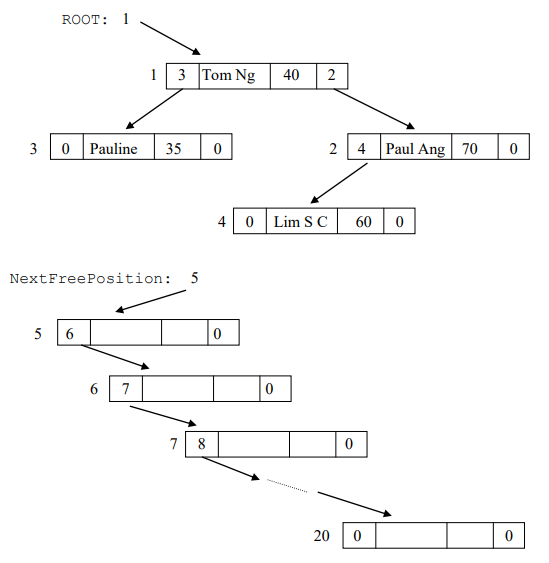
\includegraphics[width=0.65\paperwidth]{C:/Users/Admin/Desktop/Github/question_bank/LyX/static/img/9597-HCI-2015-P1-Q4-1}
\par\end{center}

The diagram shows the binary tree with the students\textquoteright{}
scores 40, 70, 35 and 60 (added in that order) and linked list of
unused nodes after the four students\textquoteright{} scores have
been added. 

\subsection*{Task 4.1 }

Write the program code to declare all the required variables and create
the initial linked list which contains all 20 nodes. Add statement(s)
to initialize the empty tree. 

\subsection*{Evidence 17: }

Your program code for Task 4.1. {[}8{]} 

The following (incomplete) pseudocode inserts a student\textquoteright s
name and his/her score into the binary tree structure. 

The \texttt{LastMove} variable holds the direction of the previous
traversal move as follows: 

X -{}- no move yet made 

L -{}- move was to the left

R -{}- move was to the right 

\noindent %
\noindent\begin{minipage}[t]{1\columnwidth}%
\texttt{PROCEDURE AddNodeToBinaryTree(NewName, NewScore) \bigskip{}
}

\texttt{IF Root = 0 }

\texttt{\qquad{}THEN }

\texttt{\qquad{}\qquad{}Root <- NextFreePosition }

\texttt{\qquad{}ELSE }

\texttt{\qquad{}\qquad{}//traverse the tree to find the position
for the new value }

\texttt{\qquad{}\qquad{}CurrentPosition <- Root }

\texttt{\qquad{}\qquad{}LastMove <- \textquoteleft X\textquoteright{} }

\texttt{\qquad{}\qquad{}REPEAT}

\texttt{\qquad{}\qquad{}\qquad{}PreviousPosition <- CurrentPosition }

\texttt{\qquad{}\qquad{}\qquad{}IF NewScore < ThisTree{[}CurrentPosition{]}.Score }

\texttt{\qquad{}\qquad{}\qquad{}\qquad{}THEN }

\texttt{\qquad{}\qquad{}\qquad{}\qquad{}\qquad{}//move left }

\texttt{\qquad{}\qquad{}\qquad{}\qquad{}\qquad{}LastMove <- \textquoteleft L\textquoteright{} }

\texttt{\qquad{}\qquad{}\qquad{}\qquad{}\qquad{}CurrentPosition
\textleftarrow{} ThisTree{[}CurrentPosition{]}.LeftP }

\texttt{\qquad{}\qquad{}\qquad{}\qquad{}ELSE}

\texttt{\qquad{}\qquad{}\qquad{}\qquad{}\qquad{}// move right }

\texttt{\qquad{}\qquad{}\qquad{}\qquad{}\qquad{}LastMove <- \textquoteleft R\textquoteright{} }

\texttt{\qquad{}\qquad{}\qquad{}\qquad{}\qquad{}CurrentPosition
\textleftarrow{} ThisTree{[}CurrentPosition{]}.RightP }

\texttt{\qquad{}\qquad{}\qquad{}ENDIF }

\texttt{\qquad{}UNTIL CurrentPosition = 0}

\texttt{ENDIF \bigskip{}
}

\texttt{IF LastMove = \textquoteleft R\textquoteright{} }

\texttt{\qquad{}THEN }

\texttt{\qquad{}\qquad{}ThisTree{[}PreviousPosition{]}.RightP <-
NextFreePosition }

\texttt{\qquad{}ELSE }

\texttt{\qquad{}\qquad{}ThisTree{[}PreviousPosition{]}.LeftP <-
NextFreePosition}

\texttt{ENDIF }

\texttt{NextFreePosition \textleftarrow{} ThisTree{[}NextFreePosition{]}.LeftP\bigskip{}
}

\texttt{ENDPROCEDURE }%
\end{minipage}

Note: The above text is available in the text file \texttt{PSEUDOCODE\_TASK\_4\_2.txt} 

\subsection*{Task 4.2 }

Write non-recursive code to implement the \texttt{AddNodeToBinaryTree}
procedure that will add a new node with student\textquoteright s name
and score into the binary tree structure. 

You may use the text file \texttt{PSEUDOCODE\_TASK\_4\_2.txt} as a
basis for the writing of your code. 

The given pseudocode is incomplete as: 
\begin{itemize}
\item it does not initially test that there is free node available for a
new student 
\item it does not assign \texttt{NewName} and \texttt{NewScore} to the data
fields of the \texttt{ThisTree} array Add these requirements to your
program solution.
\end{itemize}

\subsection*{Evidence 18: }

Your program code for Task 4.2. \hfill{} {[}6{]}

\subsection*{Task 4.3 }

Write a procedure \texttt{OutputData} which displays the value of
\texttt{Root}, the value of \texttt{NextFreePosition} and the contents
of \texttt{ThisTree} in index order.

\subsection*{Evidence 19: }

Your program code for Task 4.3. \hfill{}{[}5{]}

\subsection*{Task 4.4 }

Write a main program to: construct a binary search tree using the
data provided in the text file \texttt{SCORES.txt} by calling procedure
\texttt{AddNodeToBinaryTree} . Your program will then call procedure
\texttt{OutputData}. 

\subsection*{Evidence 20: }

Your program code for Task 4.4. \hfill{}{[}3{]}

\subsection*{Evidence 21:}

Screenshot showing the output from running the program in Task 4.4
\hfill{}{[}5{]}

\subsection*{Task 4.5 }

Write a recursive procedure \texttt{RankList} to output the students\textquoteright{}
names and scores in descending scores order. Include a call to the
procedure from your main program. Evidence 22: Your program code for
Task 4.5. {[}6{]} 

\subsection*{Evidence 23: }

Provide a screenshot showing students\textquoteright{} names and scores
in descending scores order. \hfill{} {[}2{]}